\begin{figure}[h]
  %\centering
  \begin{tabular}{ p{2.5cm} p{2.6cm} p{3.7cm} p{2.5cm} }
     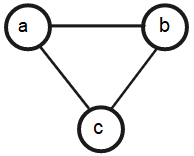
\includegraphics[width=2.3cm, left]{./img/trianguloabc.png} & 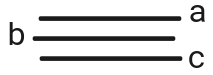
\includegraphics[width=2.5cm]{./img/b0epgtriangulo.png} & 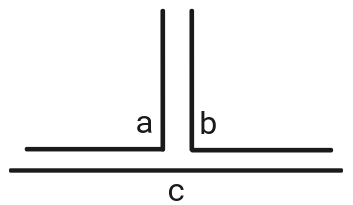
\includegraphics[width=3.5cm, left]{./img/b1epgtriangulo.png} & 
  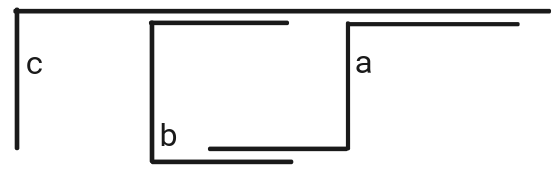
\includegraphics[width=5cm]{./img/b2epgtriangulo.png}\\%[\abovecaptionskip]
    \footnotesize (a) The $C_3$ graph & \footnotesize(b) $B_0$-EPG($C_3$)  & \footnotesize \centering (c) $B_1$-EPG($C_3$)  &  \footnotesize  (d) $B_2$-EPG($C_3$) \\
 \footnotesize & \footnotesize \centering representation & \centering  \footnotesize representation  & \footnotesize \centering representation\\  
  \end{tabular}
  %\vspace{2cm}  
%segundo bloco de figuras
%   \begin{tabular}{r p{2.5cm} @{}c@{} }
%     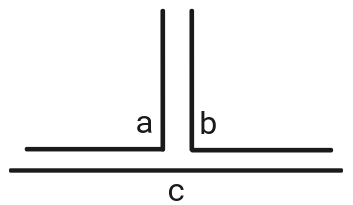
\includegraphics[width=4cm]{./img/b1epgtriangulo.png} & &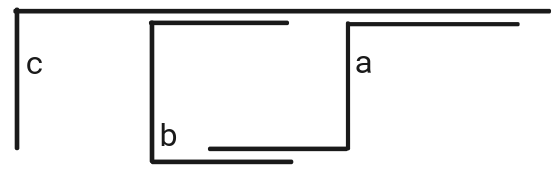
\includegraphics[width=6cm]{./img/b2epgtriangulo.png}  \\%[\abovecaptionskip] 
%     \footnotesize (c) Representação $B_1$-EPG($C_3$) & & \footnotesize (d) Representação $B_2$-EPG($C_3$)
%   \end{tabular}
 \caption{The $ C_3 $ graph  and some representations: without bend, with 1 bend and with 2 bends} \label{fig:trianguloepgRepresentacao}
\end{figure}